\section{Exponential Distribution ( $\text{Exponential}(\lambda)$ )}


\begin{table}[H]
    \hfill
    \begin{minipage}{0.45\linewidth}
        \begin{figure}[H]
            \centering
            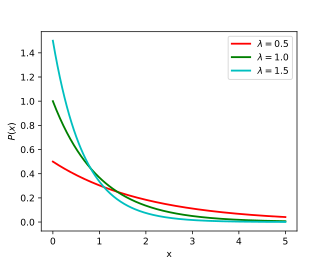
\includegraphics[
                width=\linewidth,
                height=5cm,
                keepaspectratio,
            ]{images/distributions/Exponential_distribution_pdf_-_public_domain.svg.png}
            \caption{Exponential Distribution: PDF \cite{wiki/Exponential_distribution}}
        \end{figure}
    \end{minipage}
    \hfill
    \begin{minipage}{0.45\linewidth}
        \begin{figure}[H]
            \centering
            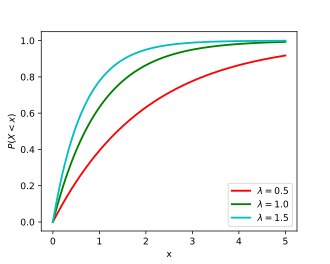
\includegraphics[
                width=\linewidth,
                height=5cm,
                keepaspectratio,
            ]{images/distributions/Exponential_distribution_cdf_-_public_domain.svg.png}
            \caption{Exponential Distribution: CDF \cite{wiki/Exponential_distribution}}
        \end{figure}
    \end{minipage}
    \hfill
\end{table}



\subsection{Distribution of the Sample Statistic ($T_n$)}

\begin{enumerate}
    \item Let $X_1 , X_2, \cdots , X _n$ are i.i.d. exponentially distributed, i.e. $X _i \sim \exp(\lambda )$.
    \hfill \cite{statistics/book/Statistics-for-Data-Scientists/Maurits-Kaptein}

    \item The exponential distribution function is given by $F (x) = 1 - \exp (-\lambda x)$ for $x > 0$ and zero otherwise.
    \hfill \cite{statistics/book/Statistics-for-Data-Scientists/Maurits-Kaptein}
\end{enumerate}

\subsubsection{Distribution of the Sample Minimum ($T_n = F _{X_{(1)}}$)}

\begin{enumerate}
    \item $F _{X_{(1)}} (x) = 1 - \exp (-n\lambda x)$ for $x > 0$ and zero otherwise
    \hfill \cite{statistics/book/Statistics-for-Data-Scientists/Maurits-Kaptein}

    \item Thus this implies that the sample distribution of the minimum $X_{(1)}$ is exponentially distributed, $X_{(1)} \sim \exp (n\lambda)$, but now with parameter $n\lambda$, when $X_1 ,X_2, \cdots , X _n$ are i.i.d. $\exp(\lambda)$ distributed.
    \hfill \cite{statistics/book/Statistics-for-Data-Scientists/Maurits-Kaptein}
\end{enumerate}



\subsection{Summary}

\begin{enumerate}
    \item \textbf{Parameters}: ${\displaystyle \lambda >0}$ (rate or inverse scale)
    \hfill \cite{wiki/Exponential_distribution, statistics/book/Statistics-for-Data-Scientists/Maurits-Kaptein}

    \item \textbf{Support}: ${\displaystyle x\in [0,\infty )}$
    \hfill \cite{wiki/Exponential_distribution, statistics/book/Statistics-for-Data-Scientists/Maurits-Kaptein}

    \item \textbf{PDF}:
    ${\displaystyle \lambda e^{-\lambda x}}$
    \hfill \cite{wiki/Exponential_distribution, statistics/book/Statistics-for-Data-Scientists/Maurits-Kaptein}

    \item \textbf{CDF}: ${\displaystyle 1-e^{-\lambda x}}$
    \hfill \cite{wiki/Exponential_distribution}

    \item \textbf{Quantile}: ${\displaystyle -{\dfrac {\ln(1-p)}{\lambda }}}$
    \hfill \cite{wiki/Exponential_distribution}

    \item \textbf{Mean}: $\dfrac{1}{\lambda}$
    \hfill \cite{wiki/Exponential_distribution}

    \item \textbf{Median}: $\dfrac{\ln(2)}{\lambda}$
    \hfill \cite{wiki/Exponential_distribution}

    \item \textbf{Mode}: $0$
    \hfill \cite{wiki/Exponential_distribution}

    \item \textbf{Variance}: $\dfrac{1}{\lambda^2}$
    \hfill \cite{wiki/Exponential_distribution}

    \item \textbf{Skewness}: $2$
    \hfill \cite{wiki/Exponential_distribution}

    \item \textbf{Excess kurtosis}: $6$
    \hfill \cite{wiki/Exponential_distribution}

    \item \textbf{Entropy}: $1-\ln(\lambda)$
    \hfill \cite{wiki/Exponential_distribution}

    \item \textbf{Fisher information}: $\dfrac{1}{\lambda^2}$
    \hfill \cite{wiki/Exponential_distribution}

    \item \textbf{Expected shortfall}:
    $
        {\displaystyle {\dfrac {-\ln(1-p)+1}{\lambda }}}
    $
    \hfill \cite{wiki/Exponential_distribution}

    \item \textbf{Moment-generating function (MGF)}:
    $
        {\displaystyle {\dfrac {\lambda }{\lambda -t}},{\text{ for }}t<\lambda }
    $
    \hfill \cite{wiki/Exponential_distribution}

    \item \textbf{Characteristic function (CF)}:
    $
        {\displaystyle {\dfrac {\lambda }{\lambda -it}}}
    $
    \hfill \cite{wiki/Exponential_distribution}

    \item \textbf{Kullback–Leibler divergence}:
    $
        {\displaystyle \ln {\dfrac {\lambda _{0}}{\lambda }}+{\dfrac {\lambda }{\lambda _{0}}}-1}
    $
    \hfill \cite{wiki/Exponential_distribution}
\end{enumerate}





















